\subsection{Notation}
\TODO{Notation needs to be introduced in the background section, Tiling should be the first subsection}
We represent a decision tree by $T = (V, E, r)$ where $V$ is the set of nodes, $E$ the set of edges and
$r \in V$ is the root. For each node $n \in V$, we define the following.
\begin{enumerate}
    \item $threshold(n) \in \mathbb{R}$, the threshold value for $n$.
    \item $featureIndex(n) \in \mathbb{N}$, the feature index for $n$.
    \item $left(n) \in V$, the left child of $n$ or $\emptyset$ if $n$ is a leaf. If $left(n) \neq \emptyset$, then $(n, left(n)) \in E$.
    \item $right(n) \in V$, the right child of $n$ or $\emptyset$ if $n$ is a leaf. If $right(n) \neq \emptyset$, then $(n, right(n)) \in E$.
\end{enumerate}
We use $L \subseteq V$ to denote the set of leaves. % subseteq because tree could have single node

\subsection{Tiling}
\label{sec:Tiling}
% Treebeard vectorizes tree walks by grouping nodes of a decision tree into \textbf{\emph{tiles}}. The nodes in a tile are evaluated concurrently using vector instructions. Once the nodes of the current tile are evaluated, a look up table is used to compute which child of the current tile to move to next.

While a decision tree is naturally represented by a binary tree, 
it is not the best representation for tree traversal as it (i) requires many memory accesses, 
(ii) has poor branching structure and (iii) cannot make use of vector instructions. 
This section proposes a tiling optimization where we group multiple nodes in a decision tree into a single tile, effectively transforming a binary tree into an $n$-ary tiled tree. This not only allows the compiler to generate vectorized code (see Section~\ref{sec:Vectorization} ) to traverse trees but also enables spatial locality improvements by grouping nodes that are likely to be accessed together. We demonstrate this with two tiling heuristics later in the section. 



\CommentOut{
Treebeard groups nodes of the decision tree into \textbf{\emph{tiles}}. Tiling provides two benefits. 
\begin{enumerate}
  \item It allows the compiler to generate vector code to traverse trees. Section \ref{sec:Vectorization} describes how Treebeard does this.
  \item It enables spatial locality improvements by grouping together nodes that are likely to be accessed together. 
\end{enumerate}
Once nodes are grouped into tiles, an $n$-ary tree whose nodes are tiles is constructed. Treebeard then generates 
optimized code to walk this tree. The listing below shows at a high level how a tiled tree is walked (This is not 
true IR, but presented for clarity). 
}

Once trees are tiled Treebeard generates tree walks with the code structure shown below.
\begin{lstlisting}[style=c++]
  ResultType Prediction_Function(...) {
    // ...
    Tile t = getRootTile(tree)
    while (!isLeaf(tree, t)) do {
      // Evaluate conditions of all nodes in the tile
      predicates = evaluateTilePredicates(t, rows[i])
      
      // Move to the correct child of the current tile
      t = getChildTile(tree, t, predicates) 
    }
    treePrediction = getLeafValue(t)
    // ...
  }  
\end{lstlisting}
The code is just an abstract representation of a tiled tree walk that enables efficient lowering of specific steps in subsequent stages. 
\op{evaluateTilePredicates} (speculatively) computes the predicates on all nodes in a tile (line 6). Then \op{getChildTile} (line 9), uses the computed predicate values to determine which child of the current tile to move to. We defer a description of how these operators are lowered to a later section but focus on tiling algorithms in this section.

\CommentOut{
To compute the prediction of the tree, the predicates of all nodes in the tile are computed simultaneously (line 6). 
Then, the computed predicate values are used to determine which child of the current tile to move to (in the 
$n$-ary tree). This section presents the details of tiling and how Treebeard's general tiling infrastructure 
can be used to develop tiling algorithms with different objectives (sections \ref{sec:UnifTiling}) and \ref{sec:ProbTiling}).
The details of how Treebeard lowers predicate evaluation and moving to the correct child to use vector instructions 
are described in section \ref{sec:Vectorization}.

\subsection{Tiles and Tree Tiling}
\label{sec:ValidTiling}
}
\subsection*{Conditions for Efficient Tiling}
\label{sec:ValidTiling}
While any arbitrary partitioning of the nodes of a tree could be considered for tiling we impose a few intuitive constraints.
% to only allow nodes that are likely to be accessed together to be grouped into a tile. 
\TODO{kr : replace $n_t$ with sz?}
Given a $tree = (V, E, r)$ and a tile size $n_t$ we impose the following constraints on the generated tiles $\{ T_1, T_2, ... ,T_m \}$ .
\begin{description}
    \item[Partitioning] $T_1 \cup T_2 ... \cup T_m = V$ and $T_i \cap T_j = \emptyset$ for all $i\neq j$
    \item[Connectedness] If $u, v \in T_i$, there is a (undirected) path connecting $u$ and $v$ fully contained in $T_i$.
   \item [Leaf seperation] $\forall l \in L$ : $l \in T_i \rightarrow v \notin T_i \;\; \forall v \in V \backslash \{l\}$
  \item [Maximal tiling] if there are tiles such that. $|T_i| < n_t$ then there is no $v \in V\backslash \{ T_i \cup L \}$ such that $(u, v) \in E$ for some $u \in T_i$. 
\end{description}
The \textbf{partitioning} and \textbf{maximal tiling} constraints together ensure that we group nodes into as few tiles as possible. {\textbf{Connectedness}} ensures that each tile is a sub-tree, a natural grouping of nodes that are likely to be accessed together. The {\textbf{Leaf separation}} constraint ensures that leafs are not tiled along with internal nodes. Leafs in a decision tree need special handling, they are used to check for walk termination and to determine the output (prediction). This constraint ensures that tiles are homogenous, this in-turn allows us to specialize the in-memory layout of trees and also simplifies code generation. We discuss leaf handling and tree layout in Section~\ref{sec:}.
We refer to any tiling that satisties the above constraints as a \emph{valid} tilling.
\CommentOut{
\subsection{Tiled Trees}
A tiling transformation communicates the tiling to the Treebeard infrastructure by assigning a tile ID to each node in the decision tree. Using these tile IDs, Treebeard checks the validity of the tiling and then contructs a tree whose nodes are tiles. We call this tree the \textbf{\emph{tree of tiles}}. \TODO{We need a better name for this}
Figure \ref{Fig:ValidTilingTileSize3} shows a valid tiling with tile size 3 and the tree of tiles constructed by Treebeard. Three nodes are grouped into each of the tiles $t_1$ and $t_2$ as shown. Each tile is collapsed into a single node in the tree of tiles. However, each leaf in the original tree becomes a leaf in the tree of tiles.

\begin{figure}
  \centering
  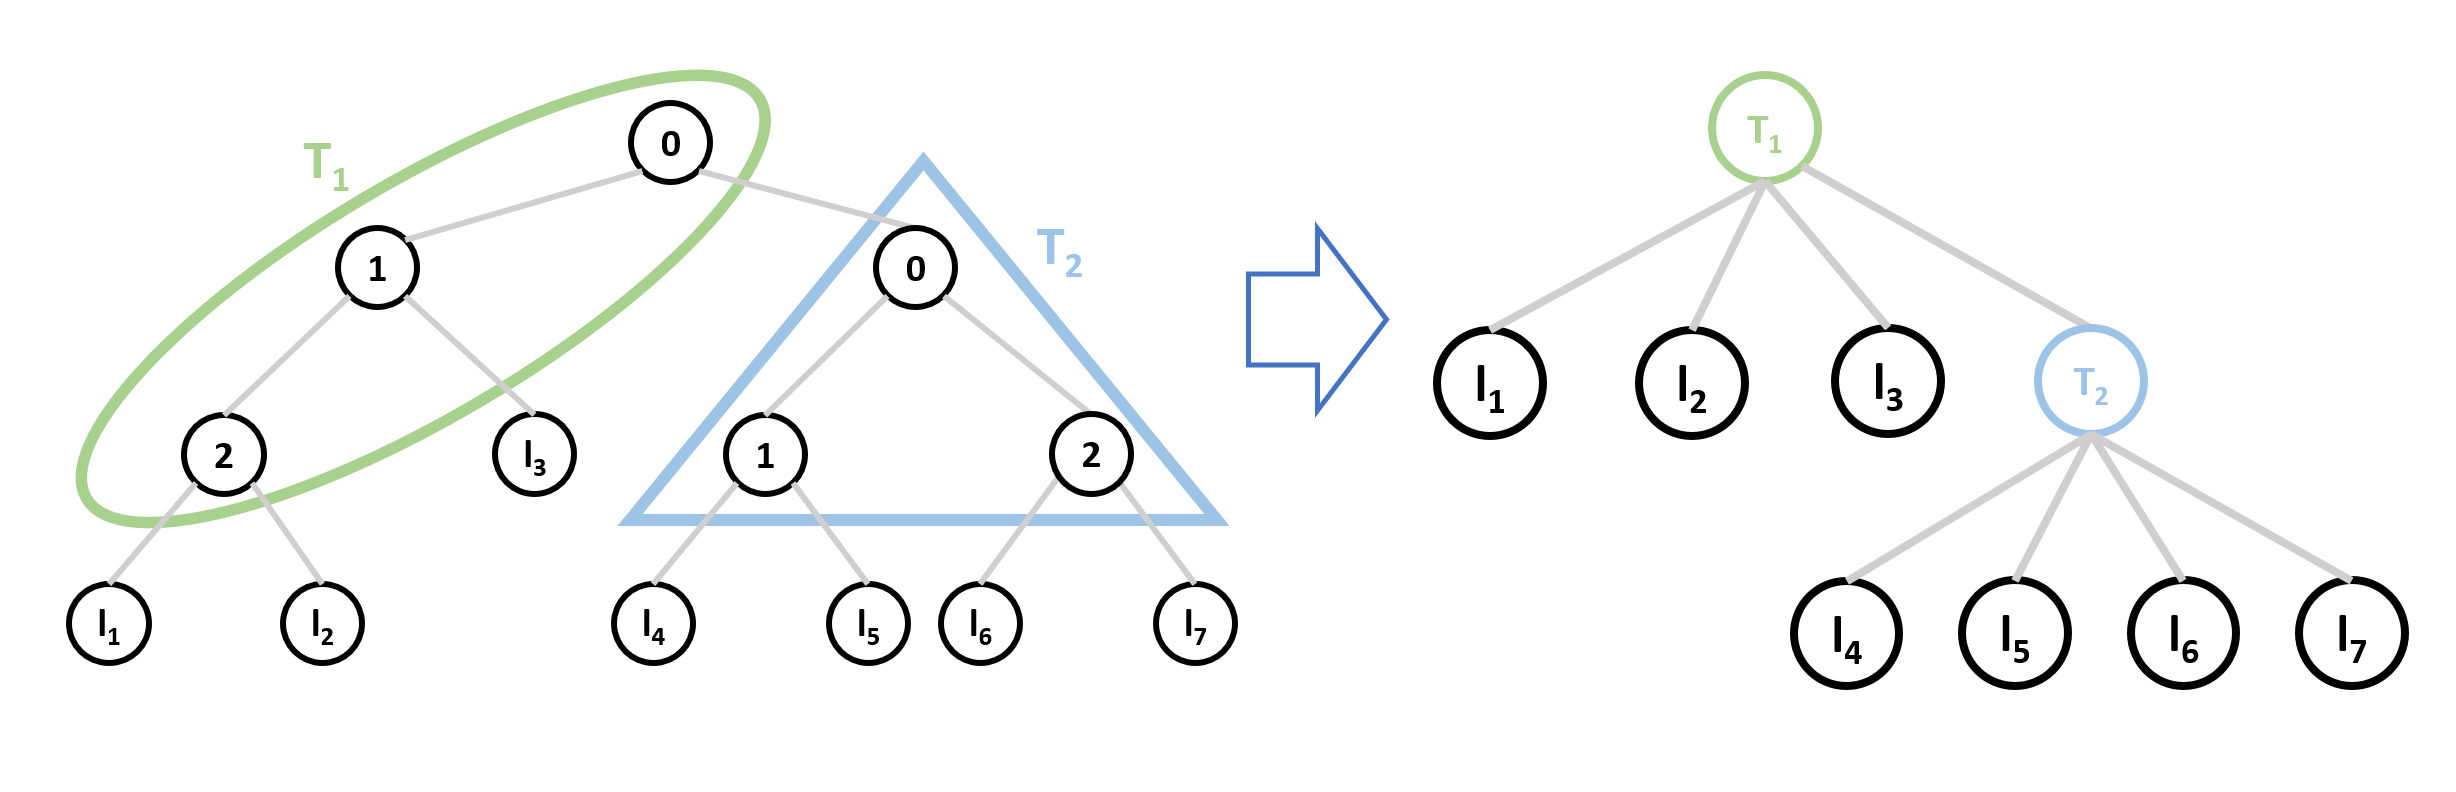
\includegraphics[width=\linewidth]{figures/TiledTree_Size3.PNG}
  \caption{Example of a valid tree tiling with tile size $n_t=3$}
  \label{Fig:ValidTilingTileSize3}
\end{figure}

Treebeard maintains the following invariants.
\begin{enumerate}
  \item All tiles in a tree are the same size $n_t$. If the tiling produces any smaller tiles, these are padded by inserting dummy nodes to make them the required size.
  \item Nodes within tiles are always ordered in level order and left to right within a level. The numbering of the nodes in the above diagram shows this node order.
  \item Children of a node are numbered from left to right (regardless of level). For example, $l_1$ is the first child of $t_1$, $l_2$ is the second and so on.
\end{enumerate}
   }
